\documentclass{article}
    % General document formatting
    \usepackage[margin=0.7in]{geometry}
    \usepackage[parfill]{parskip}
    \usepackage[utf8]{inputenc}
    
    % Related to math
    \usepackage{amsmath,amssymb,amsfonts,amsthm}
\usepackage{tikz}
\usepackage{subfigure}
\usetikzlibrary{bayesnet}

\begin{document}




\begin{figure}[ht]
  \begin{center}
    \begin{tabular}{cc}
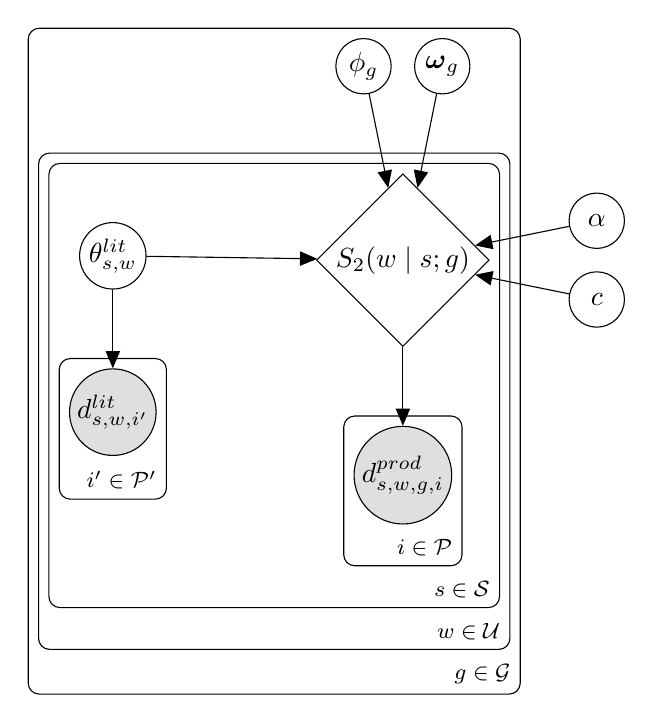
\begin{tikzpicture}



  \node[obs]          (d-prod)   {$d^{prod}_{s, w, g, i}$}; %
  \node[det, above=of d-prod]  (s2)   {$S_2(w \mid s; g)$}; %
  \edge{s2}{d-prod};
  
    \node[obs, left=2.5 of d-prod, yshift=0.8cm] (d-lit)   {$d_{s,w, i'}^{lit}$}; %
  \node[latent, above=of d-lit](lit){$\theta^{lit}_{s,w}$};%
  \edge{lit}{d-lit}
  
  \node[latent, above=of s2, xshift=0.5cm](weights){$\boldsymbol{\omega}_g$};%
  \node[latent, right=of s2, yshift=0.5cm](sopt){$\alpha$};
  \node[latent, right=of s2, yshift=-0.5cm](cost){$c$};
  \node[latent, above=of s2, xshift=-0.5cm](s1phi){$\phi_g$};
  \edge{weights}{s2};
  \edge{sopt}{s2};
  \edge{cost}{s2};
  \edge{s1phi}{s2};
  \edge{lit}{s2};
      \plate{lit-data}{
    (d-lit)
  }{$i' \in \mathcal{P}'$}
  
    \plate{prod-data}{
    (d-prod)
  }{$i \in \mathcal{P}$}
{%\tikzset{plate caption/.append style={below right=0pt and 0pt of #1.north west}}

  \plate{lit-sem}{
  (prod-data)
  (d-lit)(lit)(lit-data)
    (s2)(d-prod)
  }{$s \in \mathcal{S}$}
    \plate{lit-sem2}{
      (prod-data) (lit-data)
  (d-lit)(lit)(lit-sem)
    (s2)(d-prod)
  }{$w \in \mathcal{U}$}
        \plate{goal}{
          (prod-data)(lit-sem)(lit-sem2)
  (s2)(d-prod)(weights)(s1phi)
  }{$g \in \mathcal{G}$}
  }
  
\end{tikzpicture}

    \end{tabular}
  \end{center}
  \caption{ Bayesian data analysis model to infer RSA model parameters and generate model predictions. RSA model ($S_2$) predicts the utterance production data ($d^{prod}$) for each utterance $w$, state $s$, goal $g$, and participant $i$. The RSA model relies upon the literal semantics of each utterance for each state $\theta^{lit}$ $P(x^d_k)$, constrained by the data from the literal semantics task $d^{lit}$ (see Supplement). The $S_2$ model generates predictions given goal weights $\boldsymbol{\omega_g}$ and intended social weight $\phi_g$, which varies by the goal condition $g$. RSA model has two global free parameters: the speaker optimality parameter $\alpha$ and the utterance cost of negation $c$.}
  \label{fig:bayesnet}
\end{figure}




\end{document}

